\chapter{Symbolic knowledge representation}

\section{Challenges of this thesis}
\label{sect|krs-challenges}

First, we want to represent knowledge and not only information.  Both knowledge and information are contextualized. Knowledge also has a \emph{cultural} context that enable interpretation. 

Then, we want to make use of this representation to extend the robot's \emph{communication function} and \emph{decision function}.

Those two broad targets should lead to two improvements for human-robot interaction:
\begin{itemize}
	\item to loosen the constraints on symbolic modelling of the robot environment by providing more expressive representation system than classical databases or fact repositories,
	\item to improve human-robot interaction by explicitely providing to the machine an interpretation frame, at least partially shared with the human.
\end{itemize}

\begin{figure}%[!ht]
\centering
  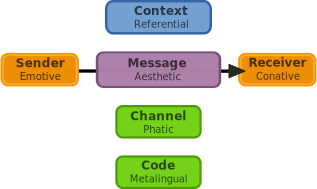
\includegraphics[width=0.6\linewidth]{communication/jakobson_communication_model.pdf}
  \caption{The \emph{Communication Model}, as proposed by Jakobson. In bold characters are the \emph{communication dimensions}, in italics, the corresponding \emph{communication functions}.}
  \label{fig|jakobson_communication_model}
\end{figure}


The operational targets are two-fold:
\begin{inparaenum}[\itshape a\upshape)]
\item determine, for a abstract/theoritical/general point of view, how and why a cognitive architecture could contribute to these aims; and
\item implement it.
\end{inparaenum}

\section{Which end for knowledge representation?}
\label{sect|krs-purpose}

\subsection{Limits of traditional representation systems for robotics}
\label{subssect|limits}

\subsection{Specific requirements of robotics}
\label{subssect|robotics-specifics}

\subsection{Benefits of a symbolic knowledge representation system}
\label{subssect|krs-benefits}

\section{Formalisms for symbolic representation}
\label{sect|formalisms}

\section{Designing the \textsc{OpenRobots} common-sense ontology}
\label{sect|commonsense-design}

\section{Evaluation of a symbolic representation }
\label{sect|krs-evaluation}

